\documentclass[10pt,aspectratio=169]{beamer}
\usetheme{AnnArbor}

% Customizing AnnArbor to use a Green palette
\usecolortheme{spruce}
\setbeamercolor{title}{bg=green!60!black,fg=white}
\setbeamercolor{frametitle}{bg=green!60!black,fg=white}
\setbeamercolor{structure}{fg=green!60!black}
\setbeamercolor{palette primary}{bg=green!60!black,fg=white}
\setbeamercolor{palette secondary}{bg=green!70!black,fg=white}
\setbeamercolor{palette tertiary}{bg=green!80!black,fg=white}
\setbeamercolor{palette quaternary}{bg=black,fg=white}
\setbeamercolor{item}{fg=green!60!black}

\usepackage{amsmath}
\usepackage{tikz}
\usepackage{graphicx}
\usetikzlibrary{positioning, arrows.meta, shapes.geometric, calc}

\title[Hospital Chatbot]{Hospital Chatbot for Color Coded Clinical Pathways}
\author{Quaigraine Samuel \and Twum Samuel}
\date{\today}

\begin{document}
	
	\begin{frame}
		\titlepage
	\end{frame}
	
	\begin{frame}{Table of Contents}
		\tableofcontents
	\end{frame}
	
	\section{Natural Language Processing}
	
	\begin{frame}{The Nuance of Human Conversation}
		\begin{center}
			% Using the specified placeholder image name 'convo'
			% Ensure 'convo.jpg' or 'convo.png' is in the same directory when compiling
			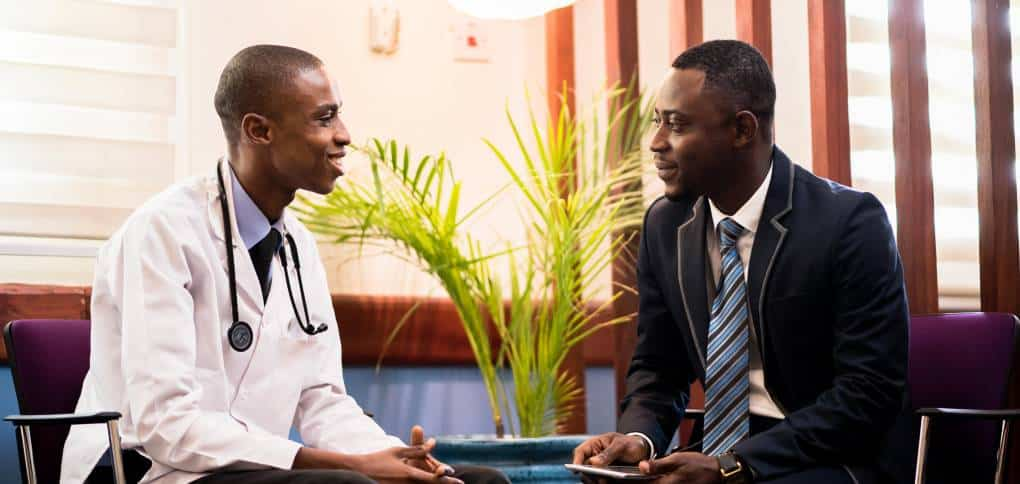
\includegraphics[height=0.6\textheight]{convo} \\
			\vspace{0.4cm}
			\Large \textit{"Human communication is inherently complex, unstructured, and contextual."}
		\end{center}
	\end{frame}
	
	\begin{frame}{Natural Language Processing (NLP) \& NLU}
		\begin{itemize}
			\item \textbf{The Core Foundation:} NLP is the foundational language engine of the hospital chatbot.
			\item \textbf{Sub-branch:} We utilize Natural Language Understanding (NLU) combined with Text Classification.
			\item \textbf{Natural Language:} The messy, unstructured way humans communicate (e.g., subjective patient symptom descriptions).
			\item \textbf{Processing Phase:} Human text is translated into rigid mathematical structures (matrices and vectors). This allows a computer to read, process, and analyze the subjective input objectively.
		\end{itemize}
	\end{frame}
	
	\begin{frame}{Aligning NLP with Clinical Standards}
		\begin{itemize}
			\item \textbf{Clinical Standard:} The South African Triage Scale (SATS) forms the backbone of our pathways.
			\item \textbf{Objective Validation:} The Triage Early Warning Score (TEWS) provides a deterministic, mathematical safety net based on vitals.
			\item \textbf{The Chatbot's Role:} By combining NLP with TEWS, the system effectively translates subjective, unstructured human complaints into objective mathematical scores that align directly with established SATS triage pathways.
		\end{itemize}
	\end{frame}
	
	\section{Machine Learning \& Neural Networks}
	\begin{frame}{Basic Machine Learning Concepts}
		\begin{columns}[T]
			\begin{column}{0.48\textwidth}
				\textbf{Types of Learning}
				\begin{itemize}
					\item \textbf{Supervised Learning:} Uses labeled data to teach the algorithm using known examples (e.g., historical triage records).
					\item \textbf{Unsupervised Learning:} Discovers hidden patterns independently in unlabeled data.
				\end{itemize}
			\end{column}
			\begin{column}{0.48\textwidth}
				\textbf{Types of Models}
				\begin{itemize}
					\item \textbf{Classification Models:} Predict distinct categories (e.g., SATS color tiers).
					\item \textbf{Regression Models:} Predict continuous numerical values.
				\end{itemize}
			\end{column}
		\end{columns}
		\vspace{0.5cm}
		\textbf{Examples:} K-Nearest Neighbors, Support Vector Machines (SVM), Decision Trees, and \textbf{Neural Networks}.
	\end{frame}
	
	\begin{frame}{Visualizing Machine Learning Models}
		\begin{columns}
			% Classification
			\begin{column}{0.33\textwidth}
				\centering
				\textbf{Classification (Supervised)} \\
				\vspace{0.2cm}
				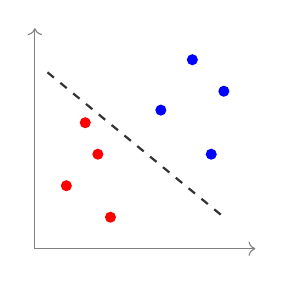
\begin{tikzpicture}[scale=0.8]
					\draw[->, gray] (0,0) -- (3.5,0);
					\draw[->, gray] (0,0) -- (0,3.5);
					\fill[red] (0.5, 1) circle (2.5pt); \fill[red] (1.2, 0.5) circle (2.5pt);
					\fill[red] (1, 1.5) circle (2.5pt); \fill[red] (0.8, 2) circle (2.5pt);
					\fill[blue] (2.5, 3) circle (2.5pt); \fill[blue] (3, 2.5) circle (2.5pt);
					\fill[blue] (2.8, 1.5) circle (2.5pt); \fill[blue] (2, 2.2) circle (2.5pt);
					\draw[thick, dashed, black!80] (0.2, 2.8) -- (3, 0.5);
				\end{tikzpicture}
			\end{column}
			% Regression
			\begin{column}{0.33\textwidth}
				\centering
				\textbf{Regression (Supervised)} \\
				\vspace{0.2cm}
				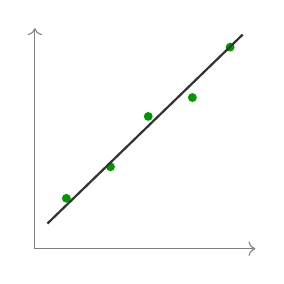
\begin{tikzpicture}[scale=0.8]
					\draw[->, gray] (0,0) -- (3.5,0);
					\draw[->, gray] (0,0) -- (0,3.5);
					\fill[green!60!black] (0.5, 0.8) circle (2pt); \fill[green!60!black] (1.2, 1.3) circle (2pt);
					\fill[green!60!black] (1.8, 2.1) circle (2pt); \fill[green!60!black] (2.5, 2.4) circle (2pt);
					\fill[green!60!black] (3.1, 3.2) circle (2pt);
					\draw[thick, black!80] (0.2, 0.4) -- (3.3, 3.4);
				\end{tikzpicture}
			\end{column}
			% Clustering
			\begin{column}{0.33\textwidth}
				\centering
				\textbf{Clustering (Unsupervised)} \\
				\vspace{0.2cm}
				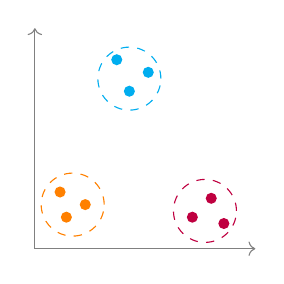
\begin{tikzpicture}[scale=0.8]
					\draw[->, gray] (0,0) -- (3.5,0);
					\draw[->, gray] (0,0) -- (0,3.5);
					\fill[orange] (0.5, 0.5) circle (2.5pt); \fill[orange] (0.8, 0.7) circle (2.5pt); \fill[orange] (0.4, 0.9) circle (2.5pt);
					\draw[orange, dashed] (0.6, 0.7) circle (0.5cm);
					\fill[purple] (2.5, 0.5) circle (2.5pt); \fill[purple] (2.8, 0.8) circle (2.5pt); \fill[purple] (3.0, 0.4) circle (2.5pt);
					\draw[purple, dashed] (2.7, 0.6) circle (0.5cm);
					\fill[cyan] (1.5, 2.5) circle (2.5pt); \fill[cyan] (1.8, 2.8) circle (2.5pt); \fill[cyan] (1.3, 3.0) circle (2.5pt);
					\draw[cyan, dashed] (1.5, 2.7) circle (0.5cm);
				\end{tikzpicture}
			\end{column}
		\end{columns}
	\end{frame}
	
	\begin{frame}{Why Neural Networks?}
		\begin{itemize}
			\item \textbf{The Limitation of Standard ML:} Traditional machine learning algorithms struggle with the immense complexity, sequential nature, and nuance of human language.
			\item \textbf{The Neural Advantage:} Neural networks excel at Natural Language Processing because they can automatically discover hidden, non-linear relationships.
			\item \textbf{Abstract Features:} Deep, stacked layers inside the network mathematically transform raw text vectors into deep semantic representations without requiring manual feature extraction.
		\end{itemize}
	\end{frame}
	
	\begin{frame}{Diagram: Neural Network Architecture}
		\begin{center}
			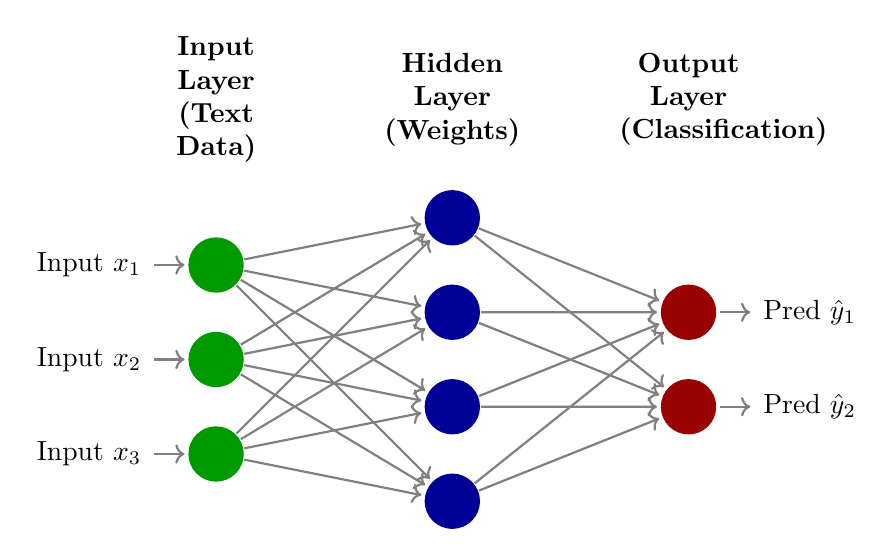
\begin{tikzpicture}[shorten >=1pt,->,draw=black!50, node distance=2.5cm, thick]
				\tikzstyle{every pin edge}=[<-,shorten <=1pt]
				\tikzstyle{neuron}=[circle,fill=black!25,minimum size=20pt,inner sep=0pt]
				\tikzstyle{input neuron}=[neuron, fill=green!60!black, text=white]
				\tikzstyle{output neuron}=[neuron, fill=red!60!black, text=white]
				\tikzstyle{hidden neuron}=[neuron, fill=blue!60!black, text=white]
				\tikzstyle{annot} = [text width=5em, text centered, font=\bfseries]
				
				% Inputs
				\foreach \name / \y in {1,...,3}
				\node[input neuron, pin=left:Input $x_\y$] (I-\name) at (0,-\y*1.2) {};
				
				% Hidden Layer
				\foreach \name / \y in {1,...,4}
				\path[yshift=0.6cm] node[hidden neuron] (H1-\name) at (3cm,-\y*1.2) {};
				
				% Output Layer
				\foreach \name / \y in {1,...,2}
				\path[yshift=-0.6cm] node[output neuron, pin={[pin edge={->}]right:Pred $\hat{y}_\y$}] (O-\name) at (6cm,-\y*1.2) {};
				
				% Edges I -> H1
				\foreach \source in {1,...,3}
				\foreach \dest in {1,...,4}
				\path (I-\source) edge (H1-\dest);
				
				% Edges H1 -> O
				\foreach \source in {1,...,4}
				\foreach \dest in {1,...,2}
				\path (H1-\source) edge (O-\dest);
				
				% Annotations
				\node[annot,above of=H1-1, node distance=1.5cm] (hl) {Hidden Layer\\(Weights)};
				\node[annot,left of=hl, node distance=3cm] {Input Layer\\(Text Data)};
				\node[annot,right of=hl, node distance=3cm] {Output Layer\\(Classification)};
			\end{tikzpicture}
		\end{center}
	\end{frame}
	
	\begin{frame}{Why Not Traditional Models?}
		\begin{itemize}
			\item \textbf{Linear Regression:} Designed exclusively to predict \textit{continuous numerical values}. It mathematically cannot predict discrete SATS triage categories (Red, Orange, Yellow).
			\item \textbf{Logistic Regression:} While it predicts categories, it assumes inputs are linear and independent. It fails to capture complex syntactic dependencies.
			\item \textbf{The NLP Failure Point:} These methods rely on basic ``Bag of Words'' counts. They completely lose the sequence and context of language, failing to differentiate the profound semantic difference between \textit{``my chest is NOT tight''} and \textit{``my chest IS tight''}.
		\end{itemize}
	\end{frame}
	
	\begin{frame}{The Math of Neural Networks: Forward \& Penalty}
		Every neural network executes a strict 4-step mathematical loop to learn.
		\vspace{0.3cm}
		\begin{block}{1. The Forward Pass (The Guess)}
			\[ y = Wx + b \]
			Transforms independent input data ($x$) into a dependent prediction ($y$) using internal weights ($W$) and biases ($b$).
		\end{block}
		\vspace{0.1cm}
		\begin{block}{2. Cross-Entropy Loss (The Penalty)}
			\[ \mathcal{L} = -\sum_{i=1}^{C} y_i \log(\hat{y}_i) \]
			If the dependent output is wrong, this calculates the exact mathematical penalty. Because of the negative log, predicting the wrong triage category with high confidence results in a massive mathematical penalty ($\mathcal{L}$).
		\end{block}
	\end{frame}
	
	\begin{frame}{The Math of Neural Networks: Investigation \& Correction}
		\begin{block}{3. Backpropagation (The Investigation)}
			\[ \frac{\partial \mathcal{L}}{\partial W} = \frac{\partial \mathcal{L}}{\partial \hat{y}} \cdot \frac{\partial \hat{y}}{\partial z} \cdot \frac{\partial z}{\partial W} \]
			Uses the Chain Rule of calculus to travel backward through the network. It calculates the exact gradient (the slope of the error) to determine which specific weights caused the bad guess.
		\end{block}
		\vspace{0.1cm}
		\begin{block}{4. Optimization (The Correction)}
			\[ W_{new} = W_{old} - \alpha \left( \frac{\partial \mathcal{L}}{\partial W} \right) \]
			Using Gradient Descent, the algorithm physically adjusts the weights ($W$) in the opposite direction of the gradient by a step size defined by the Learning Rate ($\alpha$).
		\end{block}
	\end{frame}
	
	\section{Transformers \& BERT}
	\begin{frame}{Transformers: Revolutionizing NLP}
		\begin{itemize}
			\item \textbf{The Problem:} Standard ML and early neural networks struggled with long text because they read words sequentially (one by one).
			\item \textbf{The Breakthrough:} The 2017 \textit{"Attention Is All You Need"} paper introduced the Transformer architecture.
			\item \textbf{Parallel Processing:} Transformers abandoned sequential reading, allowing the model to read and process entire sentences in parallel.
		\end{itemize}
	\end{frame}
	
	\begin{frame}{Diagram: The Self-Attention Mechanism}
		\begin{center}
			% THE FIX: Constrain the image to 80% of the slide's maximum height
			\resizebox{!}{0.8\textheight}{%
				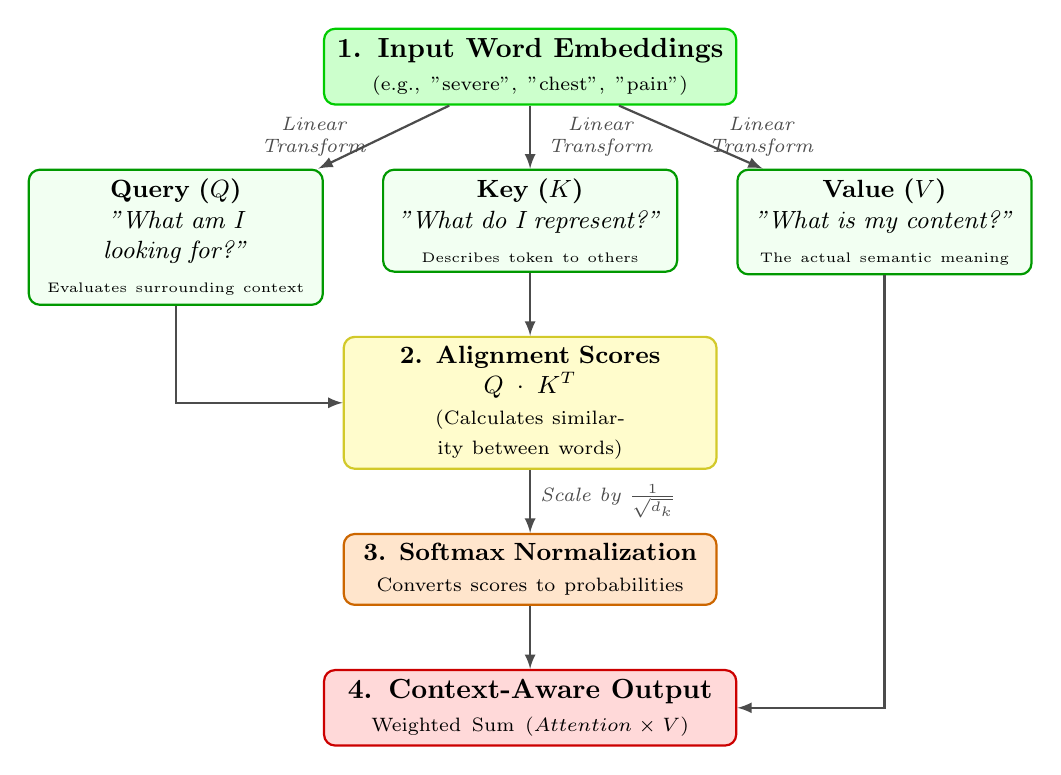
\begin{tikzpicture}[node distance=0.8cm, thick,
					box/.style={draw=green!60!black, rectangle, fill=green!5, text width=3.5cm, align=center, minimum height=0.9cm, rounded corners, font=\small},
					highlightbox/.style={draw=green!80!black, rectangle, fill=green!20, text width=5cm, align=center, minimum height=0.8cm, rounded corners, font=\bfseries},
					arrow/.style={->, >=latex, thick, draw=black!70},
					label/.style={font=\scriptsize\itshape, text=black!70, align=center}
					]
					
					% Top Input
					\node[highlightbox] (input) {1. Input Word Embeddings\\ \mdseries \scriptsize (e.g., "severe", "chest", "pain")};
					
					% Q, K, V Splits
					\node[box, below=0.8cm of input, xshift=-4.5cm] (query) {\textbf{Query ($Q$)}\\ \textit{"What am I looking for?"} \\ \vspace{0.05cm} \tiny Evaluates surrounding context};
					\node[box, below=0.8cm of input] (key) {\textbf{Key ($K$)}\\ \textit{"What do I represent?"} \\ \vspace{0.05cm} \tiny Describes token to others};
					\node[box, below=0.8cm of input, xshift=4.5cm] (value) {\textbf{Value ($V$)}\\ \textit{"What is my content?"} \\ \vspace{0.05cm} \tiny The actual semantic meaning};
					
					% Alignment Scores
					\node[box, fill=yellow!20, draw=yellow!80!black, below=0.8cm of key, text width=4.5cm] (matmul) {\textbf{2. Alignment Scores}\\ $Q \cdot K^T$ \\ \mdseries \scriptsize (Calculates similarity between words)};
					
					% Softmax
					\node[box, fill=orange!20, draw=orange!80!black, below=0.8cm of matmul, text width=4.5cm] (softmax) {\textbf{3. Softmax Normalization}\\ \mdseries \scriptsize Converts scores to probabilities};
					
					% Final Output
					\node[highlightbox, fill=red!15, draw=red!80!black, below=0.8cm of softmax, text width=5cm] (output) {\textbf{4. Context-Aware Output}\\ \mdseries \scriptsize Weighted Sum ($Attention \times V$)};
					
					% Arrows
					\draw[arrow] (input) -- node[label, left, xshift=-0.1cm] {Linear\\Transform} (query);
					\draw[arrow] (input) -- node[label, right, xshift=0.1cm] {Linear\\Transform} (key);
					\draw[arrow] (input) -- node[label, right, xshift=0.1cm] {Linear\\Transform} (value);
					
					\draw[arrow] (query) |- (matmul);
					\draw[arrow] (key) -- (matmul);
					
					\draw[arrow] (matmul) -- node[label, right] {Scale by $\frac{1}{\sqrt{d_k}}$} (softmax);
					
					\draw[arrow] (softmax) -- (output);
					\draw[arrow] (value) |- (output);
					
				\end{tikzpicture}
			}
		\end{center}
	\end{frame}
	
	\begin{frame}{The Mathematics of Self-Attention}
		The self-attention matrix calculates exactly how much words relate to each other:
		
		\begin{block}{Self-Attention Formula}
			\[ \text{Attention}(Q,K,V) = \text{softmax}\left(\frac{QK^T}{\sqrt{d_k}}\right)V \]
		\end{block}
		\begin{itemize}
			\item \textbf{Independent Variables:} Queries ($Q$), Keys ($K$), and Values ($V$).
		\end{itemize}
		\vspace{0.2cm}
		\begin{block}{Softmax Weighting}
			\[ a_j = \frac{\exp(e_j)}{\sum \exp(e_k)} \]
		\end{block}
		\begin{itemize}
			\item \textbf{Dependent Variable:} The final Attention Weight ($a_j$). It depends entirely on the raw mathematical scores of the surrounding words, mathematically assigning massive weight to critical triage keywords.
		\end{itemize}
	\end{frame}
	
	\begin{frame}{BERT: Bidirectional Encoder Representations}
		\begin{itemize}
			\item \textbf{Bidirectionality:} Pre-machine learning models and early NLP read text strictly left-to-right. BERT reads context from both the left and the right simultaneously to deeply understand semantic meaning.
			\item \textbf{Pre-Training via MLM:} BERT learns the language through Masked Language Modeling. 
			\item \textbf{The Process:} It randomly hides 15\% of the words in a sentence and attempts to guess them based on the surrounding context.
		\end{itemize}
	\end{frame}
	
	\begin{frame}{BERT Pre-Training Mathematics}
		\begin{block}{Masked Language Modeling Loss}
			\[ \mathcal{L}_{LM} = -\sum \log P(t_i | H^{(L)}; \theta) \]
		\end{block}
		\vspace{0.5cm}
		\begin{itemize}
			\item \textbf{Independent Variables ($H^{(L)}$):} The surrounding, unmasked context words the model is allowed to read.
			\item \textbf{Dependent Variable ($\mathcal{L}_{LM}$):} The loss penalty. The penalty size depends entirely on the probability ($P$) the model assigned to the correct hidden word.
		\end{itemize}
	\end{frame}
	
	\section{BioBERT \& Classification}

\begin{frame}{BioBERT \& Triage Classification}
	\begin{columns}[T]
		% Slightly widened text column for better readability
		\begin{column}{0.55\textwidth}
			\begin{itemize}
				\item \textbf{Training Data:} Pre-trained on millions of PubMed Biomedical Abstracts, providing deep, pre-existing intuition for medical jargon.
				\item \textbf{Processing:} Text is pushed through 12 neural layers to generate a compressed summary.
				\item \textbf{Independent Variable:} The \texttt{[CLS]} token—a 768-dimensional mathematical vector summarizing the complaint.
				\item \textbf{Dependent Variable:} The model multiplies this 768-dim vector by custom weights to predict the SATS triage category.
			\end{itemize}
		\end{column}
		
		% Image column
		\begin{column}{0.45\textwidth}
			\begin{center}
				% THE FIX: Constrain diagram height so it perfectly fits the column
				\resizebox{!}{0.75\textheight}{%
					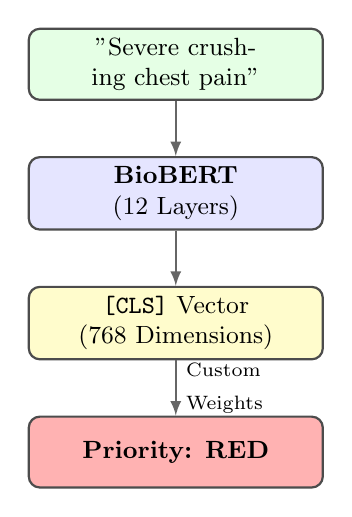
\begin{tikzpicture}[node distance=0.7cm, auto, thick,
						box/.style={draw=black!70, rectangle, fill=green!10, text width=3.5cm, align=center, minimum height=0.9cm, rounded corners, font=\small},
						arrow/.style={->, >=latex, thick, draw=black!60}]
						
						\node[box] (input) {"Severe crushing chest pain"};
						\node[box, fill=blue!10, below=of input] (biobert) {\textbf{BioBERT}\\ (12 Layers)};
						\node[box, fill=yellow!20, below=of biobert] (vector) {\texttt{[CLS]} Vector \\(768 Dimensions)};
						\node[box, fill=red!30, below=of vector] (output) {\textbf{Priority: RED}};
						
						\draw[arrow] (input) -- (biobert);
						\draw[arrow] (biobert) -- (vector);
						\draw[arrow] (vector) -- node[right, text width=1.5cm, align=left] {\scriptsize Custom\\Weights} (output);
					\end{tikzpicture}
				}
			\end{center}
		\end{column}
	\end{columns}
\end{frame}

\section{Data Engineering \& Performance}

\begin{frame}{The Training Data: Sources \& Statistical Profile}
	\begin{columns}[T]
		\begin{column}{0.55\textwidth}
			\begin{itemize}
				\item \textbf{Data Provenance:}Pre-trained on 18B words from PubMed/PMC and Fine-tuned on the \textbf{Triagegeist Dataset} (synthetic, 80k records). This allows us to model ED statistics with \textbf{zero privacy risk}.
				\item \textbf{Statistical Distribution:}
				\begin{itemize}
					\item \textbf{Mode (Most Frequent):} Level 3 (Yellow) at 36.15\%.
					\item \textbf{Median:} Level 3, representing a moderate baseline.
					\item \textbf{Rarest Class:} Level 1 (Red) at just 4.03\%.
				\end{itemize}
				\item \textbf{The Imbalance Ratio:} There is a $\sim$9:1 ratio between the mode (most frequent) and the most critical emergency class.
			\end{itemize}
		\end{column}
		
		\begin{column}{0.45\textwidth}
			\vspace{0.2cm}
			\textbf{Distribution of 80,000 Records} \\
			\vspace{0.2cm}
			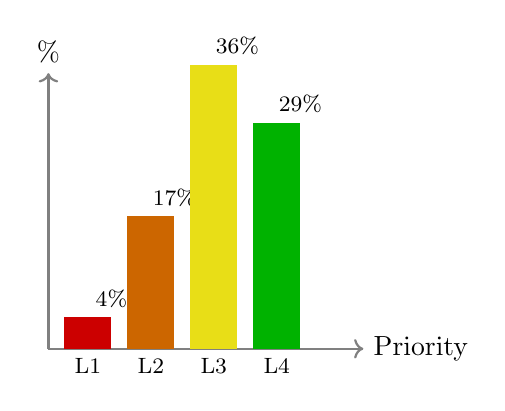
\begin{tikzpicture}
				\draw[->, thick, gray] (0,0) -- (4,0) node[right, black] {Priority};
				\draw[->, thick, gray] (0,0) -- (0,3.5) node[above, black] {\%};
				
				\fill[red!80!black] (0.2,0) rectangle (0.8,0.4) node[above, black] {\footnotesize 4\%};
				\node[below] at (0.5,0) {\footnotesize L1};
				
				\fill[orange!80!black] (1.0,0) rectangle (1.6,1.68) node[above, black] {\footnotesize 17\%};
				\node[below] at (1.3,0) {\footnotesize L2};
				
				\fill[yellow!90!black] (1.8,0) rectangle (2.4,3.61) node[above, black] {\footnotesize 36\%};
				\node[below] at (2.1,0) {\footnotesize L3};
				
				\fill[green!70!black] (2.6,0) rectangle (3.2,2.87) node[above, black] {\footnotesize 29\%};
				\node[below] at (2.9,0) {\footnotesize L4};
			\end{tikzpicture}
		\end{column}
	\end{columns}
\end{frame}

\begin{frame}{How Data Statistics Shape Model Performance}
	\begin{itemize}
		\item \textbf{Gradient Dominance:} Because the mode (Level 3) and Level 4 make up $\sim$65\% of the training data, the neural network's loss gradient naturally prioritizes learning these common cases.
		\item \textbf{Clinical Grounding (TEWS \& SATS):} To overcome the risk of the model over-relying on text alone, the BioBERT training was mathematically anchored to objective TEWS and SATS labels.
		\begin{itemize}
			\item \textit{The Effect:} This gives the text embeddings "clinical intuition" by forcing them to correlate with actual physical vital signs.
		\end{itemize}
		\item \textbf{Final Architecture:} By combining this TEWS-aligned medical triage model with a deterministic TEWS fallback system, we overcome statistical biases and ensure that critical, life-threatening cases are never missed.
	\end{itemize}
\end{frame}
	
\end{document}